\documentclass[10pt,a4paper]{article}
\usepackage[margin=2.2cm]{geometry}
\usepackage{fontspec}
\usepackage{kotex}
\setmainfont{Apple SD Gothic Neo}
\setsansfont{Apple SD Gothic Neo}
\usepackage{amsmath,amssymb}
\usepackage{graphicx}
\usepackage{caption}
\usepackage[dvipsnames]{xcolor}
\usepackage[colorlinks=true,linkcolor=MidnightBlue,citecolor=MidnightBlue,
            urlcolor=MidnightBlue]{hyperref}
\usepackage{titlesec}
\titleformat{\section}{\large\bfseries}{\thesection}{0.6em}{}
\captionsetup{font=small,labelfont=bf}
\setlength{\parskip}{0.35em}
\setlength{\parindent}{0pt}
\usepackage{mdframed}
\newmdenv[linewidth=0.4pt,linecolor=gray!60,backgroundcolor=gray!5,
          innertopmargin=6pt,innerbottommargin=6pt,skipabove=8pt,skipbelow=8pt]{claimbox}
\newcommand{\claim}[2]{\begin{claimbox}\textbf{주장.} #1\par\smallskip
  \textcolor{gray!70}{\textbf{반증 조건.} #2}\end{claimbox}}

\title{\bfseries 전이는 이름을 지우자 강해졌다\\[2pt]
\large 두 전이 자의 화해 --- 그리고 `창 없음'($843$)과 `라우팅'($851$)의 동시 재작성}
\author{월드모델 실험실 · 노트 $852$}
\date{2026-08-09}
\begin{document}\maketitle

\section{한 줄}

티처 \#$17$ 이 잡았다: $843$ 은 전이 $0.2969$ 위에, $851$ 은 앵커 $0.3919$
위에 서 있었고 --- 같은 평가 $322$행의 두 자가 화해된 적이 없었다. 같은
$12$씨앗 적합 \textbf{한 벌}에서 예측 경로만 갈라 쟀다:
\textbf{만화-정체 예측(A) $\rho$ $0.2561$ 대 무정체 OOC 예측(B) $0.3919$ ---
격차 $+0.1358$ 이 순수 예측 경로다}(B와 $848$ 앵커의 예측 상관 $1.0000$).
KR 행에 `만화'라는 이름을 붙이는 것이 $-0.136$ 만큼 해롭다.

\begin{figure}[t]\centering
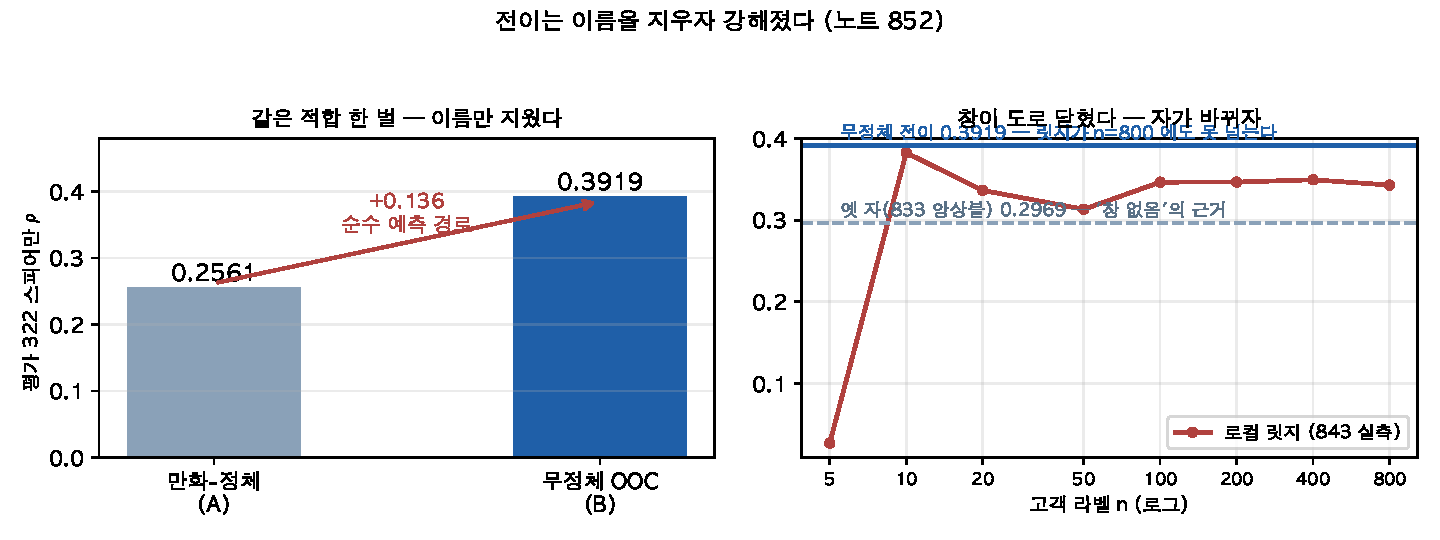
\includegraphics[width=0.97\textwidth]{figs/nameless.pdf}
\caption{왼쪽: 같은 적합, 이름만 지웠다. 오른쪽: 자가 바뀌자 $843$ 의 릿지
곡선이 어느 $n$ 에서도 전이를 못 넘는다.}
\end{figure}

\claim{\textbf{세 서사가 한 번에 다시 쓰였다.} ① 전이 상수의 정본 =
\textbf{무정체(OOC) 경로 $0.3919$} --- 신규 도메인 서빙은 정체 없이.
② $843$ `창 없음($n^{\dagger}{=}10{\sim}20$)' 재서술: 그 판정은 A-류 자 위 ---
B-자로는 \textbf{릿지가 $n{=}800$ 에서도 전이를 못 넘는다}($0.343 < 0.392$).
창이 없는 게 아니라 측정 범위 내 \emph{전이 우위 지속}이다. ③ $851$ 라우팅
폐기: $n^{\ddagger}$ 는 `라벨 등록으로 하락하는 합동'이라는 잘못된 팔과의
교차였다. 처방(KR 짝): \textbf{고객 라벨을 합동에 등록하지 말고, 정체 없이
전이하라.}}
{$833$ 의 $0.2969$ 는 A 로 재현되지 않았다($0.2561$ · 차 $0.041$) ---
앙상블 구성(TabPFN 포함 여부) 조사를 미결로 등록했고, 못 닫으면 규약 $44$
(재현 불능 · 새 자) 처리다. 이것은 KR 짝 하나의 실측이다 --- 앱은 릿지
$0.51$ 이 확실히 전이 위($822$)라 도메인마다 다르고, 일반화는 같은 $4$팔
대조 후에만.}

\section{정직}

왜 이름이 해로운지(판 만화(JP)의 눈금이 KR 에 안 맞는다는 후보)는 걸지
않는다 --- 기제 예측은 $6$연속 틀렸고 순서·문턱 예측만 걸어 이번도
$2/3$(경로 격차 · 지문 적중, $833$ 재현 구간 미스). B 경로의 강함이
OOC\_DROP 보정 덕인지는 미분해. 티처 \#$17$ 의 나머지 적발(n$80$ 해부 ·
'실측 종결' 과대 · annex$5$ 타이브레이크)은 전부 미결/정정으로 등록했다.
GitHub 흐름 $12$회째. 판 $\rho$ $0.4710$ 그대로.

\end{document}
